\chapter{Debezium}
Debezium\cite{Debezium} je projekt, ktorý slúži k zaznámenavaniu zmien v databázi analýzou udalostí v transakčnom logu. Jednou z podporovaných databázi je taktiež MySQL.
Na správnu funkcionalitu Debezium potrebuje metadáta popisujúce štruktúru databáze v závislosti na čase. Pre MySQL je to možné dosiahnuť tak, že príkazy, ktoré vytvárajú alebo upravujú štruktúru databáze (DDL) sú zachytávané, parsované a na ich základe je upravený model v pamäti, ktorý popisuje štruktúru databáze. 

\section{Zachytávanie zmenených dát}
Hlavnou myšlienkou zachytávania zmenených dát, anglicky \nomExpl{CDC}{Change Data Capture}, je vytvárať sled událostí, ktoré reprezentujú všetky zmeny v tabulkách danej databáze. To znamená, že pre každý \textit{insert}, každý \textit{update}, každý \textit{delete} dotaz sa vytvorí jedena odpovedajúca událosť, ktorá bude odoslaná a následne dostupná pre konzumentov tohto sledu viď obrázok \ref{fig:CDC} \cite{debezium:devoxx}. V projekte Debezium sa na sprostredkovanie sledu události využíva Apache Kafka \cite{Kafka} infraštruktúra, no myšlienka CDC nie je viazaná na Kafku.

\begin{figure}[H]
\begin{center}
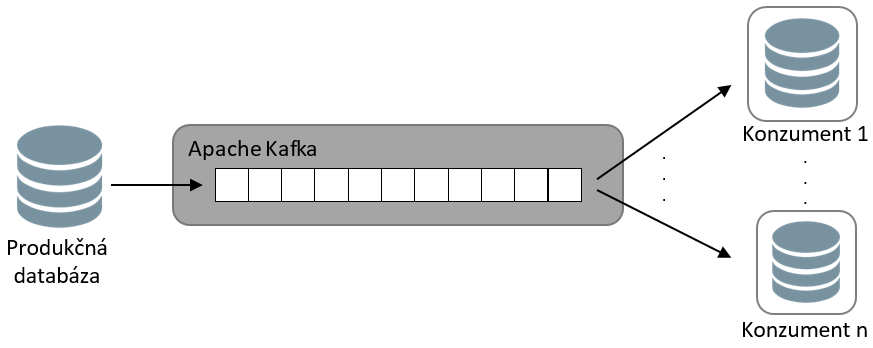
\includegraphics[width=15cm]{figures/CDC_1.PNG}
\caption{Koncept distribúcie zmenených dát}
\label{fig:CDC}
\end{center}
\end{figure}

\subsection{Dátové sklady}
% http://enos.itcollege.ee/~gseier/C__DOCUME~1_GUSTAV_LOCALS~1_TEMP_plugtmp_Attunity_CDC_White_Paper.pdf
V dátových skladoch sa uchovávajú dáta a ich história z viacerých databází za účelom analytických výpočtov. Aktuálne najpoužívanejším riešením na napĺňanie dátových skladov je ETL\footnote{Export, transform, load}. Tento proces funguje v zmysle periodického nahrávania veľkého množstva dát do dátových skladov. Tento proces sebou ale nesie nevýhody, ktoré v minulosti neboli tak podstatné, no v dnešnej dobe už sú. Použitím CDC miesto ETL je možné niektoré z týchto nevýhod obmedziť. Dátové sklady sa za pomoci CDC napĺňajú priebežne a nie periodicky, takže dáta nad ktorými sa vykonáva analýza budú skoro vždy aktuálne. Nakoľko sa každá zmena zapisuje jednotlivo a nie pomocou veľkého balíčku, neobmedzí to beh systémov, zamedzí nutnosti systémových prestojov a zároveň to redukuje cenu za túto operáciu. Premiestnením iba zmenených údajov CDC vyžaduje oveľa menej zdrojov na presun a transformáciu dát. To zníži náklady na hardvér, softvér a aj ľudské zdroje. \cite{attunity:etl_cdc}

\subsection{Replikácia dát}
Jedným z využití CDC je replikácia dát do iných databáz napríklad v zmysle vytvorenia zálohy dát, ale taktiež je možné CDC využíť pri implementácií zaujímavých analytických požiadavkov. Predstavme si, že máme produkčnú databázu a specializovaný analytický systém na ktorom chceme spustiť analýzu. V tomto prípade je nutné dostať dáta z produkčnej databáze do analytického systému a CDC je možnosť, ktorá nám to umožní. Ďalším využitím môže byť prísun dát ostatným týmom, ktoré na základe nich múžu napríklad vypočítavať a smerovať svoju marketingovú kampaňn napríklad na užívateľov, ktorý si objednali istý konkrétny produkt. Nakoľko necheme aby sa takýto výpočet vykonával nad produkčnou databázov ale skôr nad nejakou separovanou databázov, tak opäť je možné využiť CDC na propagáciu dát do separovanej databáze, kde si už marketingový tým môže vykonávať akokoľvek náročné výpočty.

\subsection{Microservice Architecture}
Ďalšie využitie CDC je vhodné pri použití Microservice architecture, kde je doména rozdelená na niekoľko služieb, ktoré potrebujú medzi sebou interagovať. Pre príklad máme tri micro služby: objednávaciu aplikáciu na spracovávanie užívateľských objednávok, produktovú službu, ktorá sa stará o produktový katalóg, a nakoniec máme skladovú službu, ktorá kontroluje reálne množstvo produktových vecí na sklade. Je zretelné, že na správne fungovanie bude objednávacia aplikácia vyžadovať dáta od produktovej a skladovej služby. Jednou z možností je, že objednávacia aplikácia bude priamo komunikovať s ostatnými službami napríklad pomocou REST API\footnote{\url{https://cs.wikipedia.org/wiki/Representational_State_Transfer}}, čím ale bude úzko spojená a závislá na chode danej služby. Ak by takáto služba zlyhala/spadla tak nebude fungovat celá aplikácia. Druhou možnosťou je práve využiť CDC, ktoré odzrkadľuje použitie Event Sourcing paternu\footnote{\url{http://microservices.io/patterns/data/event-sourcing.html}}. Produktová a skladová služba budú poskytovať sled zmenených dát a objednávacia aplikácia ich bude zachytávať a udržiavať kópiu časti týchto dát, ktoré ju zaujímajú, vo vlastnej lokálnej databáze. Ak by v takomto prípade niektorá zo služieb zlyhala, tak objednávacia aplikácia môže naďalej fungovať.

\subsection{Ostatné}
Bežnou praxou vo väčších aplikáciach je používanie cache pre rýchly prístup k dátam na základe špecifických dotazov. V takýchto prípdoch je potrebné riešiť problémy updatu cache alebo jej invalidácie, pokiaľ sa isté dáta zmenia.

Riešenie fulltextového vyhľadávania pomocou databáze nie je veľmi vhodné a namiesto toho sa používa SOLR\footnote{\url{http://lucene.apache.org/solr/}} alebo Elasticsearch\footnote{\url{https://www.elastic.co/}}, čo sú systémy, ktoré potrebujú byť synchronizované z dátami v primárnej databáze. 


\section{Odchytávanie zmien v databázi}
Každý databázový systém (\nom{DBMS}{Database management system}) má svoj log súbor, ktorý používa na zotavenie sa po páde a odvolani transakcií, ktoré ešte neboli potvrdené alebo na replikáciu dát voči sekundárným databázam alebo inej funkcionalite. Či už to sú transakčné, binárne alebo replikačné logy, vždy v sebe udržujú všetky transakcie, ktoré boli úspešne vykonané nad databázou, a preto sú vhodné na odchytávanie zmien v databázach pre projekt Debezium. Konkrétne v MySQL databáze sa volá \textbf{binlog} (\ref{mysql:binlog}). Nakoľko sú tieto logy plne transparentné voči aplikácií, ktorá do databáze zapisuje, výkon aplikácie nebude nijako ovplyvnený čítaním týchto logov.

\subsection{Apache Kafka}
Apache Kafka je open-source disturibuovateľná platforma na streamovanie správ vyvinutá firmou Apache Software Foundation. Umožnuje vytvárať a sledovať tok záznamov podobný fronte správ. Tento tok ukladá spôsobom odolným voči chybám. Hlavným použitím Kafky je vytváranie dátových potrubí v reálnom čase, ktoré spoľahlivo získavajú dáta medzi systémami alebo aplikáciami a budovanie aplikácií na streamovanie v reálnom čase, ktoré transformujú alebo reagujú na prúdy dát. Kafku je možné spustiť ako cluster na jednom, alebo viacerých servroch, ktoré ukladajú toky záznamov v kategóriách nazvaných \textbf{topiky}. Každá správa v Kafke pozostáva z kľúča, hodnoty a časovej značky. Každej správe Kafka priradí sekvenčné identifikačné číslo nazývané \textbf{offset}, ktoré unikátne identifikuje každý záznam a jeho poradie v topiku.

Kafka pozostáva zo štyroch základný API:\cite{Kafka}
\begin{itemize}
\item \textbf{Producer API}, ktoré umožnuje aplikáciam publikovať sled záznamov do jedného alebo viacerých topikov.
\item \textbf{Consumer API}, ktoré umožnuje konzumovať existujúce topiky a sprocesovať sled záznamov, ktorý obsahujú.
\item \textbf{Streams API}, ktoré umožnuje aplikáciam chovať sa ako spracovávateľ sledu záznamov. Aplikácie pohlcujú prichádzajúci sled a produkujú transformovaný výstupný sled.
\item \textbf{Connector API}, ktorý umožnuje vytvárať prepoužiteľné dátové spojenia na publikovanie a konzumovanie záznamov, ktoré pripoja topiky k existujúcim aplikáciám alebo dátovým systémom.
\end{itemize}

\begin{figure}[H]
\begin{center}
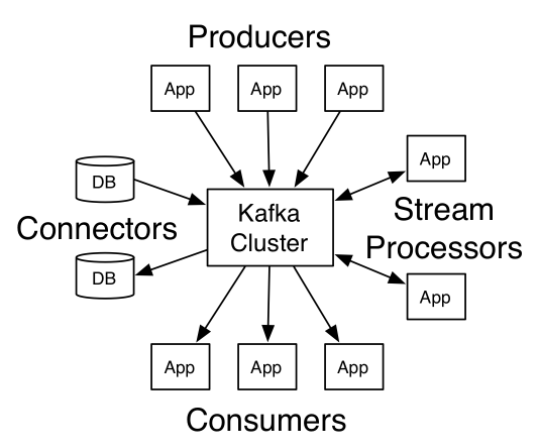
\includegraphics[width=9cm]{figures/kafka_hierarchy.PNG}
\caption{Hierarcia Apache Kafka}
\label{fig:kafka_hierarchy}
\end{center}
\end{figure}

Projekt Debezium využíva posledné zmienené \textit{Connector API} použitím Kafka Connect frameworku (\ref{kafka_connect}), pomocou ktorého implementuje CDC pre jednotlivé databázové systémy.

\subsection{Infraštruktúra správ pomocou Apache Kafka}
Apache Kafka poskytuje semantické pravidlá, ktoré dobre vyhovujú potrebám projektu Debezium. Prvým z nich je, že všetky správy v Kafke majú kľúč a hodnotu. Táto vlastnosť sa využíva na zjednotenie správ, ktoré spolu súvisia a to konkrétne tak, že na základe primárneho kľúča v tabuľke, ktorej zmena sa zmena týka je možné štruktúrovať kľúč správy a hodnota správy bude reprezentovať konkrétnu zmenu.

Kafka taktiež garantuje poradie správ metodou FIFO\footnote{First in First out}, čím sa zabezpečí správne poradie zmien, ktoré bude konzument príjmať. Táto vlastnosť je veľmi dôležitá nakoľko ak by nastala situácia \textit{insert} a následne \textit{update} alebo dve \textit{update} akcie za sebou, tak musí byť zabezpečené aby sa ku konzumentovi dostali v správnom poradí inač by mohla nastať nekonzistencia voči dátam v primárnej databáze a dátam, ktoré si udržiava konzument.

Kafka je pull-based systém, čo znamená, že konzument je sám sebe pánom a drží si informáciu o tom, ktoré správy z konkrétneho topiku už prečítal resp. kde chce začať čítanie ďalších správ. Takto môže sledovať aktuálne pribúdajúce správy, ale taktiež sa môže zaujímat aj o správy z minulosti.

Zmien v databázach môže byť veľmi veľa, čo spôsobí veľké množstvo údálosti, a preto je nutné spomnúť ďalšiu výhodu Kafky a to jej škálovateľnosť. Kafka podporuje horizontálnu škálovateľnosť a jednotivé topiky môžu byť rozdelené na viacero partícií. Je ale nutné si uvedomiť, že poradie zmien je garantované iba na konkrétnej partícii. Kafka zabezpečí, že všetky správy z rovnakým kľúčom budú na rovnakej partícii, čím sa garantuje ich správne poradie, ale môže nastať situácia, že událosť s iným kľúčom, ktorá reálne nastala neskôr, môže byt kozumentom spracovávana skôr, čo môže, ale aj nemusí vadiť v závisloti na konkrétnej funkcionalite konzumenta.

\subsection{Kafka Connect}\label{kafka_connect}
Kafka Connect je framework, ktorý umožnuje jednoduchú implementáciu dátových spojení (konektorov) s Kafkou. Tieto konektory majú na starosti dáta, ktoré vstupujú alebo vystupujú z Kafky. Nazývajú sa \textit{source}(vstupujúce dáta rep. import) konektory alebo \textit{sink}(vysupujúce dáta resp. export) konektory. Debeziové konektory majú nastarosti naplňovanie Kafky, takže sa používa \textit{source} konektor. Kafka Connect ponúka možnosť na riešenie offsetu. Narozdiel of Kafka offsetu, ktorý je priradený každej správe v topiku, Kafka Connect offset si udržuje informáciu o pozícií poslednom prečítanom evente z binlogu. Môže nastať situácia, že konektor zhvaruje a bude musieť byť reštartovaný. V takomto prípade konektor potrebuje vedieť ako ďaleko v čítani logu bol a kde má s čítaním pokračovať. 

\begin{figure}[H]
\begin{center}
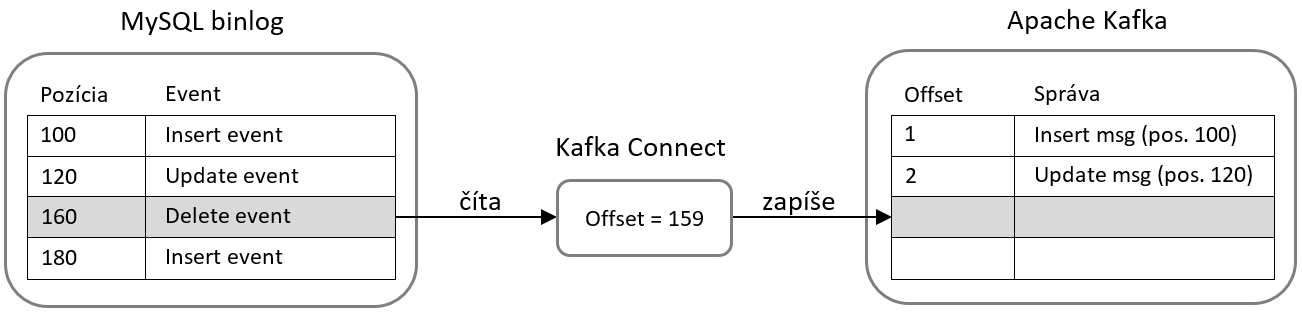
\includegraphics[width=15cm]{figures/kafka_offsets.PNG}
\caption{Príklad nastavenia Kafka a Kafka connect offsetov}
\label{fig:kafka_offsets}
\end{center}
\end{figure}

Pre príklad si povedzme, že jedna událosť v MySQL binlogu má veľkosť 20. Na obrázku \ref{fig:kafka_offsets} je možné vidieť situáciu, kedy sa konektoru podarilo prečítať a spracovať události z MySQL binlogu nachádzajúce sa na pozíciách 100 a 120. Ich príslušné správy sú dostupné v Kafke s nastaveným Kafka offsetom 1 a 2. Kafka Connect má v tejto sitácií offset rovný 159, nakoľko to je posledná prečítaná pozícia. Použitím Kafka Connect je zabezpečené, že po každom spracovaní události konektor potvrdí svoj offset a ak by konektor musel byť reštartovaný tak môže zistiť posledný potvrdený offset a pokračovať v čítaní logu z nasledujúcej pozície.

Ďalším prínosom je možnosť konfigurácie schémy správ. Kafka Connect má svoj systém na definovanie typu dát, ktorým umožnuje popísať štruktúru kľúčov a hodnôt v správach. Bližšie popísané v kapitole \ref{ssec:message_structure}.

Kafka Connect je clustrovateľná takže je možné v závislosti na špecifikácií rozdeliť konektor a jeho tasky medzi viacero uzlov. Taktiež ponúka bohatý eko-systém konektorov. Na stránkach Confluent\footnote{\url{https://www.confluent.io/product/connectors/}} je možné si stiahnuť rôzne typy či už \textit{sink} alebo \textit{source} konektorov.
Príklad CDC topológie s použitím Kafka Connect je na obrázku \ref{fig:CDC_topology} \cite{debezium:devoxx}. Zámerom v danom obrázku je zdieľať dáta dvoch tabuliek z MySQL databáze a jednej tabuľky z Postgres databáze. Každá monitorovaná tabuľka je vyjadrená jedným topikom v Kafke. Prvým krokom je nastavenie clusterov v Apache Kafka, pričom je to možné spustiť na jednom alebo viacerých clusteroch. Ďalším krokom je nastavenie Kafka Connect, ktorá je oddelená od Apache Kafka a beží v separátnych procesoch alebo clustroch, a ktorá bude spravovať spojenie z Apache Kafka. Následne je nutné nasadiť instancie Debezium konektorov do Kafka Connect a to konkrétne MySQL a Postgres konektory, nakoľko sú sledované dáta v týchto DBMS. Posledným krokom je konfigurácia aspoň jedného \textit{sink} konektoru, ktorý bude spracovávat dané topiky v Apache Kafka a odosielať ich inému systému (konzumentovi). Na konkrétnom príklade je použitý Elasticsearch konektor nakoľko je konzumentom Elasticsearch.

\begin{figure}[H]
\begin{center}
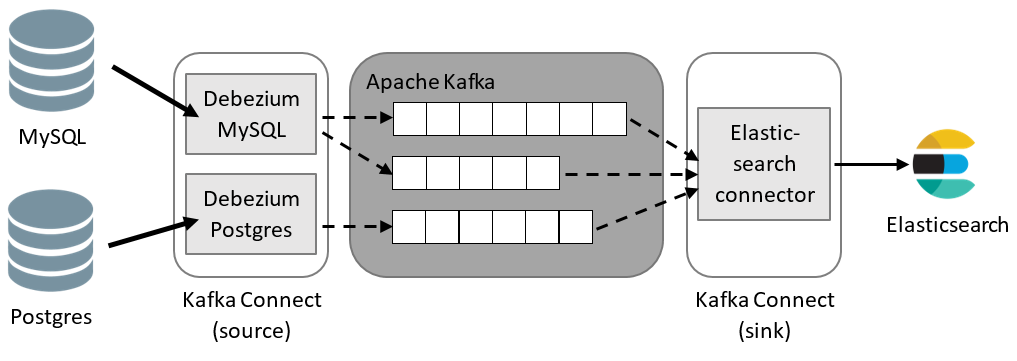
\includegraphics[width=15cm]{figures/CDC_topology.PNG}
\caption{CDC topológia z Kafka Connect}
\label{fig:CDC_topology}
\end{center}
\end{figure}

\subsection{Štruktúra správy} \label{ssec:message_structure}
Ako už bolo spomenuté, správy v Kafke obsahujú kľúč, v prípade Debezia je to primárny kľúč v tabuľke, a hodnotu, ktorá má komplexnejšiu štruktúru skladajúcu sa z:
\begin{itemize}
\item \textbf{before} stavu, ktorý v sebe nesie predchádzajúci stav data, ktoré sa mení. V prípade, že nastane \textit{insert} event, táto hodnota bude prázdna, nakoľko práve vzniká a nemá žiadny predchádzajúci stav.
\item \textbf{after} stavu, ktorý v sebe nesie nový stav dát. Táto hodnota môže byť opäť prázdna a to v prípade \textit{delete} události.
\item \textbf{source} informácie, ktoré v obsahujú metadáta o pôvode danej zmeny. Tieto dáta sú závislé na type databáze, ktorá sa sleduje. V MySQL sa napríklad skladá z informácií ako meno databázového serveru, názvu logovacieho súboru, z ktorého číta a pozíciu v ňom, názvu databáze a tabuľky, timestamp a pod.
\end{itemize}

Kafka dokáže spracovávať akýkoľvek druh textových a binárných dát, takže jej na tejto logickej štruktúre nezáleží. Na odosielanie správ sa používajú konvertory, ktoré prevádzajú správu do formy v ktorej bude odosielaná. Vďaka použitiu Kafka Connect je opäť možnosť využit konvertory, ktoré poskytuje a pre Debezium to sú:
\begin{itemize}
\item \textbf{JSON}, do ktorého je možnosť zahrnúť informácie o schéme dát, na základe ktorej môžu konzumenti správne interpretovať prijatú správu. Tento formát je výhodné používať počas vývoja aplikácie nakoľko je čitateľný pre človeka. Ukážku správy vo formáte JSON je možné zhliadnut v prílohe \ref{code:schemaExample}.
\item \textbf{Avro}, ktorý má veľmi efektívnu a kompaktnú reprezentáciu vhodnú na produkčné účely. Takáto správa nieje vo forme aby ju človek bez úprav mohol prečítal, nakoľko je to binárna reprezentácia správy. V týchto správach sa nenachádza informácia o schémy tabuľky, ale iba identifikátor na danú schému a jej verziu, ktorú je možné získať pomocou registru schémat, čo je ďalšia časť ekosystému Kafky. Konzument môže získať konkrétnu schému z registrov a na základe nej interpretovat binárne dáta, ktoré dostal.
\end{itemize}

% \subsection{Inicializácia}